\documentclass[a4paper]{book}
 
% - taille de la fonte    : 10pt, 11pt, 12pt
% - recto ou recto-verso    : oneside, twoside
 
% Chargement d'extensions
\usepackage[utf8]{inputenc}
\usepackage[T1]{fontenc}
%\usepackage[ddmmyyyy]{datetime}    


\usepackage{amssymb}
\usepackage{amsmath}
\usepackage{graphicx}
\usepackage{amscd}
\usepackage{vmargin}
\usepackage{wasysym}


\renewcommand{\contentsname}{Table des mati\`eres}  
\renewcommand{\chaptername}{Chapitre}  
 
\newtheorem{definition}{D\'efinition}
\newtheorem{proposition}{Proposition}
\newtheorem{conjecture}{Conjecture}
\newtheorem{lemma}{Lemme}
\newtheorem{proof}{Preuve}
\newtheorem{exemple}{Exemple}
\newtheorem{remark}{Remarque}
\newtheorem{theorem}{Th\'eor\`eme}
\newtheorem{corollary}{Corollaire}

\newcommand{\Rr}{\mathbb{R}}
\newcommand{\CC}{\mathbb{C}}
\newcommand{\PP}{\mathbb{P}}
\newcommand{\EE}{\mathbb{E}}
\newcommand{\HH}{\mathcal{H}}
\newcommand{\TT}{\mathbb{T}}
\newcommand{\FF}{\mathcal{F}}
\newcommand{\ve}{\varepsilon}
\newcommand{\bino}{\rm bin}
\newcommand{\NN}{\mathbb{N}}
\newcommand{\ZZ}{\mathbb{Z}}
\newcommand{\BB}{\mathcal{B}}
\newcommand{\card}{{\rm card}}
\newcommand{\jac}{{\rm Jac}}
\newcommand{\vari}{\textrm{Var}}
\newcommand{\covar}{{\rm Cov}}

\usepackage{tikz}
\usepackage{pgfplots}

\title{\Huge \bf Paragraphe à rajouter dans OPT-NNET}


 
\begin{document}
 
\section{Convexité}


\subsection{Définition}

\begin{definition}
Une fonction $f : \Rr^n \to \Rr^n$ est dite convexe si pour tous $x,y \in \Rr^n$ et tout $t \in [0,1]$ on a : $$f(tx+(1-t)y) \le t f(x) + (1-t) f(y).$$ La fonction $f$ est dite strictement convexe si pour tous $x,y \in \Rr^n$ et tout $t \in ]0,1[$ on a : $$f(tx+(1-t)y) < t f(x) + (1-t) f(y).$$
\end{definition}

En d'autres termes, la droite passant par les points de coordonnées $(x,f(x))$ et $(y,f(y))$ se situe au-dessus du graphe de la fonction $f$. On peut ainsi illustrer la convexité de la fonction "valeur absolue" $x \mapsto |x|$, ici avec $x=-3$ et $y=2$ : 

\bigskip
 
\begin{center}
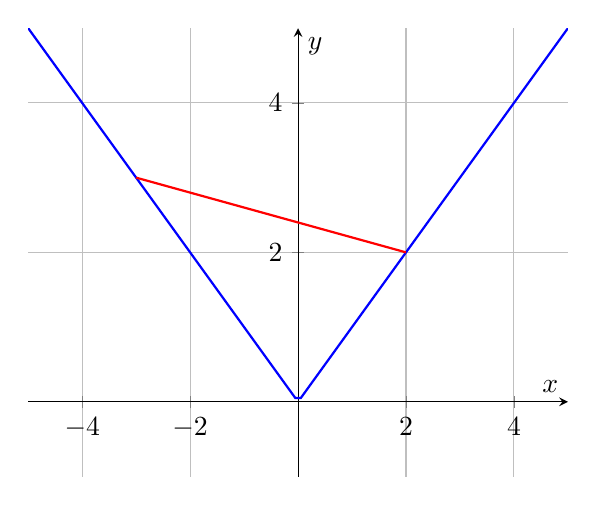
\begin{tikzpicture}
\begin{axis}[
    axis lines = middle,
    xlabel = $x$,
    ylabel = $y$,
    xmin=-5,  
 xmax=5,
    ymin=-1, ymax=5,
    grid=major,
]

\addplot[domain=-5:5, samples=100, blue, thick] {abs(x)};

% Exemple de segment pour illustrer la convexité
\addplot[red,thick] coordinates {(-3,3)(2,2)};

\end{axis}
\end{tikzpicture}
\end{center}

De la définition de convexité on en déduit l'inégalité des pentes :

\begin{proposition}
Soit $f : \Rr \to \Rr$ une fonction convexe et $x_1<x_2<x_3<x_4$ des réels. On a : $$\frac{f(x_2)-f(x_1)}{x_2-x_1} \le \frac{f(x_4)-f(x_3)}{x_4-x_3}.$$
\end{proposition}

Donnons une idée de la preuve : on pose $t = \frac{x_3-x_2}{x_3-x_1}$ et $s = \frac{x_4-x_3}{x_4-x_2}$, de telle sorte que $s,t \in [0,1]$ et : $$x_2 = (1-t)x_1+t x_3 \ , \ x_3 = (1-s) x_2+s x_4.$$ Par convexité de $f$ on a : $$f(x_2) \le (1-t) f(x_1)+t f(x_3) \ , \ f(x_3) \le (1-s) f(x_2)+s f(x_4).$$ En combinant ces deux inégalités on obtient : $$ts(f(x_4)-f(x_3)) \geq (1-t) (1-s) (f(x_2)-f(x_1)).$$ En remplaçant $s$ et $t$ par les expressions explicites et après simplifications on obtient le résultat voulu.

\subsection{Convexité et hessienne}

Une fonction convexe est toujours continue, mais pas forcément partout différentiable : pour un contre-exemple, il suffit de considérer la fonction "valeur absolue" $x \mapsto |x|$, qui n'est pas dérivable en $0$.

\bigskip

\begin{proposition}
Une fonction $f : \Rr \to \Rr$ de classe $\mathcal{C}^2$ est convexe si et seulement si sa dérivée seconde vérifie $f'' \geq 0$.
\end{proposition}

\begin{proof}
On suppose que $f$ est convexe et de classe $\mathcal{C}^2$. On veut montrer que la dérivée seconde $f''$ est à valeurs positives. Pour ce faire, on va montrer que la dérivée première $f'$ est une fonction croissante. Soient $x<y$ deux réels et $h>0$ petit. L'inégalité des pentes appliquée à $x,x+h,y,y+h$ s'écrit : $$\frac{f(x+h)-f(x)}{h} \le \frac{f(y+h)-f(y)}{h}.$$ En faisant tendre $h \to 0$, on obtient l'inégalité entre dérivées à droite $f'(x) \le f'(y)$ donc $f'$ est bien croissante.

\bigskip

Réciproquement, soit $f : \Rr \to \Rr$ de classe $\mathcal{C}^2$ vérifiant $f'' \ge 0$. Soient $x \le y \in \Rr$ et $t \in [0,1]$. On pose $z = (1-t) x + t y$, de telle sorte que $x \le z \le y$. Le théorème des accroissements finis donne l'existence de $a \in [x,z]$ et de $b \in [z,y]$ tels que $f'(a) = \frac{f(z)-f(x)}{z-x}$ et $f'(b) = \frac{f(y)-f(z)}{y-z}$. Comme $a \le b$, on a $f'(a) \le f'(b)$, donc $$(f(z)-f(x))(y-z) \le (f(y)-f(z))(z-x).$$ En remarquant que $t = \frac{z-x}{y-x}$, la dernière inégalité se transforme facilement en $f(z) \le (1-t) f(x) + t f(y)$, donc $f$ est bien convexe.
\end{proof}

On souhaite généraliser cette propriété aux fonctions à plusieurs variables. Le problème qui se présente immédiatement est que la notion de dérivée seconde se généralise en matrice hessienne.

\begin{definition}
Une matrice symétrique $H$ est dite positive, et on note $H \ge 0$, si toutes ses valeurs propres sont positives, ou de façon équivalente si on a ${}^TX H X \ge 0$ pour tout vecteur colonne $X$.
Une matrice symétrique $H$ est dite définie positive, et on note $H > 0$, si toutes ses valeurs propres sont strictement positives, ou de façon équivalente si on a ${}^TX H X > 0$ pour tout vecteur colonne $X \neq 0$. 
\end{definition}

On rappelle qu'une matrice symétrique réelle est diagonalisable dans $\Rr$ : elle possède une base de vecteurs propres associés à des valeurs propres qui sont toutes réelles.

\bigskip

Le lien entre convexité et dérivée seconde s'énonce alors comme suit : 
\begin{proposition}
Soit $f : \Rr^n \to \Rr$ une fonction de classe $\mathcal{C}^2$. La fonction $f$ est convexe si et seulement si pour tout $x \in \Rr^n$ on a $H_f(x) \ge 0$.
\end{proposition}

On peut illustrer cette propriété dans le cas d'un polynôme de degré $2$ : 

\begin{exemple}
On considère la fonction $f(x,y) = a x^2 + b xy + c y^2$. La hessienne de $f$ est constante, c'est la matrice $H = \begin{pmatrix} 2a & b \\ b & 2c \end{pmatrix}$. Les valeurs propres sont obtenues par recherche des racines du polynôme caractéristique, ce sont $$\lambda_1 = (a+c) - \sqrt{(a-c)^2+b^2} \ , \ \lambda_2 = (a+c) + \sqrt{(a-c)^2+b^2}.$$ Elles sont toutes les deux positives si et seulement si $a+c \ge 0$ et $(a+c)^2 \ge (a-c)^2+b^2$, c'est-à-dire $b^2 \le 4 ac$. Ainsi $f$ est convexe si et seulement si la trace et le déterminant de $H$ sont positifs.
\end{exemple}

Une autre famille d'exemples se rencontre assez souvent en science des données : 

\begin{exemple}
Soit $\phi : \Rr \to \Rr$ une fonction convexe. On définit la fonction $f : \Rr^n \to \Rr$ par $f(x_1,\ldots,x_n) = \sum_{i=1}^n \phi(x_i)$. La hessienne de $f$ est simple à calculer, on a : $$H_f(x_1,\ldots,x_n) = \textrm{Diag}(\phi''(x_1),\ldots,\phi''(x_n)).$$ Les valeurs propres de la matrice hessienne sont simplement les valeurs $\phi''(x_i)$, pour $1 \le i \le n$, et sont positives par convexité de $\phi$. Ainsi la fonction $f$ est convexe.
\end{exemple}


La proposition suivante permet de relier stricte convexité avec la hessienne : 
\begin{proposition}
Soit $f : \Rr^n \to \Rr$ une fonction de classe $\mathcal{C}^2$. On suppose que pour tout $x \in \Rr^n$ on a $H_f(x) > 0$. Alors la fonction $f$ est strictement convexe.
\end{proposition}

Remarquons que la réciproque n'est pas vraie : la fonction $f : x \mapsto x^2$ est strictement convexe mais on a $f''(0)=0$.

\subsection{Convexité et optimisation}

\begin{proposition}
Soit $f : \Rr^n \to \Rr$ une fonction strictement convexe. Alors $f$ possède au plus un minimum local.
\end{proposition}

\begin{proof}
On donne une idée preuve pour une fonction d'une seule variable. Supposons qu'il existe deux minimums locaux en $x_1$ et en $x_2$, avec $x_1<x_2$. On a, pour tout $t \in ]0,1[$, $f((1-t)x_1+tx_2) < (1-t) f(x_1) + t f(x_2)$. Par définition d'un minimum local, on a pour $t$ suffisamment petit, $f(x_1) \le f((1-t)x_1+tx_2)$, d'où on déduit que $f(x_2) \ge f(x_1)$. En considérant le fait que $x_2$ est un minimum local, on obtient de même que $f(x_2) \ge f(x_1)$, et donc $f(x_1)=f(x_2)$. Ainsi on a donc $f((1-t)x_1+tx_2) < f(x_1)$ pour tout $t \in ]0,1[$, ce qui, en prenant $t$ proche de $0$, contredit le fait que $x_1$ est un minimum local.
\end{proof}

Une fonction strictement convexe peut ne pas posséder de minimum local : la fonction identité $x \mapsto x$ est un contre-exemple. Mais sous certaines conditions (par exemple, si $f$ est définie sur un compact $K \subset \Rr^n$), on peut s'assurer de l'existence, donc de l'unicité, d'un minimum local, qui est alors un minimum global pour la fonction.

\bigskip

Cette propriété des fonctions strictement convexes en font des objets agréables à étudier en optimisation : un algorithme convergeant dans le cas général vers un minimum local convergerait dans ce cadre vers l'unique minimum global, ce qui est une réponse bien plus satisfaisante au problème initial.

\end{document}